\section{Anpassungen}\label{sec:anpassungen}

Dieser Abschnitt enthält alle auf Grund von Anmerkungen und Kritik nötigen Anpassungen an den bestehenden Prototypen.
Hierzu werden diese mit der selbem Überschrift wie in \autoref{sec:feedbackPraktisch} aufgelistet.
Zu jedem Punkt ist sodann textlich und bildlich eine Lösung gegeben.

\textbf{Telefonnummern:} Da für eine Übersicht der Objekte keine Telefonnummern benötigt werden entsteht hier nutzbarer Platz für andere Informationen.
Wie in \autoref{fig:feed-objekt} zu sehen, wird nun an Stelle der Telefonnummer die Adresse des Objekts angezeigt.
Aus Platzgründen fehlen jedoch PLZ und Ortsname.
Die Entscheidung für die Adresse viel, da im Zuge einer beobachteten Großdurchsuchung festgestellt wurde, dass der Meldekopf oft gedanklich Objekte und ihre Adressen verbindet.
Somit wurde die Adresse als weitere Identifikationshilfe der Übersicht hinzugefügt.

\begin{figure}[htp]
    \centering
    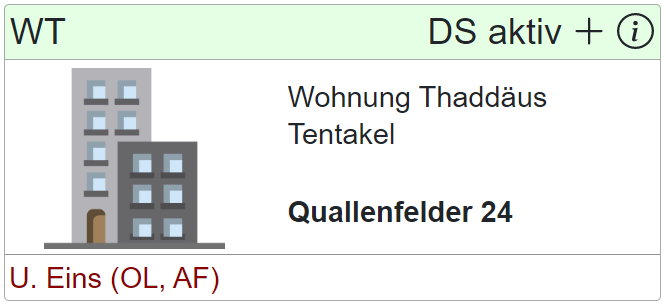
\includegraphics[width=.7\textwidth]{images/4-Feedback/objekt.png}
    \caption{Angepasste Darstellung von Objekten}
    \label{fig:feed-objekt}
\end{figure}

\textbf{Hintergrund von Objekten:} Ebenso wurde die Hintergrundfarbe von Objekten entfernt.
Hieraus resultiert eine bessere Lesbarkeit der Informationen, sowie eine gesteigerte Übersicht über alle Objekte, da die störenden Farbunterschiede wegfallen.

\textbf{Updates bearbeiten:} Updates können nun bearbeitet werden.
Hierzu kann auf das in \autoref{fig:feed-timeline} rechts zu sehende Stift-Symbol geklickt werden.
Danach ist der Text eines Updates editierbar, die Überschrift bleibt jedoch fest.
Gleichzeitig ändert sich der Stift in ein Hacken-Symbol.
Wird auf dieses geklickt, so wird der geänderte Text gespeichert und das Update kann nicht weiterbearbeitet werden.
Änderungen an einem Update werden erst im Moment des Klicks auf den Hacken mit der Datenbank synchronisiert.

\begin{figure}[htp]
    \centering
    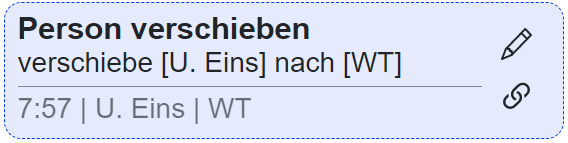
\includegraphics[width=.6\textwidth]{images/4-Feedback/timeline.png}
    \caption{Angepasste Darstellung von Updates}
    \label{fig:feed-timeline}
\end{figure}

\textbf{Timeline Tags:} Ebenso aus \autoref{fig:feed-timeline} zu erkennen ist eine neue Darstellung von Updates.
Zusätzlich zu Überschrift und Text findet sich unter diesen eine neue Zeile mit Informationen.
Hier werden die Zeit des Updates und alle in ihm erwähnten Personen, Objekte und andere Updates angezeigt.
Dieses Element fördert die Übersicht über die Timeline.
Ebenfalls eröffnet es die Möglichkeit für eine spätere tagspezifische Filterung der Timeline.

\textbf{Objekte Filtern:} Letztlich wurde die Benennung der Möglichkeit zum Filtern von Objekten angepasst.
Hier wird nun kein Filter mehr ausgewählt, es werden jedoch Tags hinzugefügt.
Damit soll den Nutzenden verdeutlicht werden, dass nur Objekte angezeigt werden, welche \textit{alle} gewählten Tags enthalten.